\chapter{Input variables with the best reconstruction improvement}
The following tables list all input variables, for which a top quark reconstruction improvement of more than \SI{4}{\%} was achieved by using the DNN classifier compared to the best-mass method introduced in Section \ref{sec:ch-4-best-mass}.

\begin{table}[h]
    \centering
    \label{tab:app_vars_1}
    \caption{Classifier input variables with which the highest reconstruction improvement was achieved.}
    \begin{tabular}{ |c|@{}c@{}| }
        \hline
        \textbf{Improvement} & \textbf{Variables}\\
        \hline
        \SI{7.83}{\%} & 
        \begin{tabular}{ll}
            \hline
            Variable & Description\\
            \hline
            $p_\text{T}\text{(j}_\text{1}$) & Transverse momentum of jet 1\\
            $\eta\text{(j}_\text{1}$) & Pseudorapidity of jet 1\\
            $\phi\text{(j}_\text{1}$) & Azimuthal angle of jet 1\\
            $m_0\text{(j}_\text{1}$) & Invariant mass of jet 1\\

            $p_T\text{(j}_\text{2}$) & Transverse momentum of jet 2\\
            $\eta\text{(j}_\text{2}$) & Pseudorapidity of jet 2\\
            $\phi\text{(j}_\text{2}$) & Azimuthal angle of jet 2\\
            $m_0\text{(j}_\text{2}$) & Invariant mass of jet 2\\

            $\Delta R \text{(j}_\text{1}\text{, W)}$ & Distance between jet 1 and the \PW boson\\
            $\Delta R \text{(j}_\text{1}\text{, lep)}$ & Distance between jet 1 and the lepton\\
            $\Delta R \text{(j}_\text{2}\text{, W)}$ & Distance between jet 2 and the \PW boson\\
            $\Delta R \text{(j}_\text{2}\text{, lep)}$ & Distance between jet 2 and the lepton\\
            \hline
        \end{tabular}\\
        \hline
    \end{tabular}
\end{table}

\begin{table}[h]
    \centering
    \label{tab:app_vars_2}
    \caption{Classifier variables that delivered the second best improvement. The \PW boson coordinates were added, the distances between the jets and the leptons were removed.}
    \begin{tabular}{ |c|@{}c@{}| }
        \hline
        \textbf{Improvement} & \textbf{Variables}\\
        \hline
        \SI{5.02}{\%} & 
        \begin{tabular}{ll}
            \hline
            Variable & Description\\
            \hline
            $p_\text{T}\text{(j}_\text{1}$) & Transverse momentum of jet 1\\
            $\eta\text{(j}_\text{1}$) & Pseudorapidity of jet 1\\
            $\phi\text{(j}_\text{1}$) & Azimuthal angle of jet 1\\
            $m_0\text{(j}_\text{1}$) & Invariant mass of jet 1\\

            $p_\text{T}\text{(j}_\text{2}$) & Transverse momentum of jet 2\\
            $\eta\text{(j}_\text{2}$) & Pseudorapidity of jet 2\\
            $\phi\text{(j}_\text{2}$) & Azimuthal angle of jet 2\\
            $m_0\text{(j}_\text{2}$) & Invariant mass of jet 2\\

            $\Delta R \text{(j}_\text{1}\text{, W)}$ & Distance between jet 1 and the \PW boson\\
            $\Delta R \text{(j}_\text{2}\text{, W)}$ & Distance between jet 2 and the \PW boson\\

            $p_\text{T}\text{(W)}$ & Transverse momentum of the \PW boson\\
            $\eta\text{(W)}$ & Pseudorapidity of the \PW boson\\
            $\phi\text{(W)}$ & Azimuthal angle of the \PW boson\\
            $m_0\text{(W)}$ & Invariant mass of the \PW boson\\
            \hline
        \end{tabular}\\
        \hline
    \end{tabular}
\end{table}

\begin{table}[h]
    \centering
    \label{tab:app_vars_3}
    \caption{Variables with the third best improvement. The distances between the jets and the lepton were added.}
    \begin{tabular}{ |c|@{}c@{}| }
        \hline
        \textbf{Improvement} & \textbf{Variables}\\
        \hline
        \SI{4.77}{\%} & 
        \begin{tabular}{ll}
            \hline
            Variable & Description\\
            \hline
            $p_\text{T}\text{(j}_\text{1}$) & Transverse momentum of jet 1\\
            $\eta\text{(j}_\text{1}$) & Pseudorapidity of jet 1\\
            $\phi\text{(j}_\text{1}$) & Azimuthal angle of jet 1\\
            $m_0\text{(j}_\text{1}$) & Invariant mass of jet 1\\

            $p_\text{T}\text{(j}_\text{2}$) & Transverse momentum of jet 2\\
            $\eta\text{(j}_\text{2}$) & Pseudorapidity of jet 2\\
            $\phi\text{(j}_\text{2}$) & Azimuthal angle of jet 2\\
            $m_0\text{(j}_\text{2}$) & Invariant mass of jet 2\\

            $\Delta R\text{(j}_\text{1}\text{, W)}$ & Distance between jet 1 and the \PW boson\\
            $\Delta R\text{(j}_\text{1}\text{, lep)}$ & Distance between jet 1 and the lepton\\
            $\Delta R\text{(j}_\text{2}\text{, W)}$ & Distance between jet 2 and the \PW boson\\
            $\Delta R\text{(j}_\text{2}\text{, lep)}$ & Distance between jet 2 and the lepton\\

            $p_\text{T}\text{(W)}$ & Transverse momentum of the \PW boson\\
            $\eta\text{(W)}$ & Pseudorapidity of the \PW boson\\
            $\phi\text{(W)}$ & Azimuthal angle of the \PW boson\\
            $m_0\text{(W)}$ & Invariant mass of the \PW boson\\
            \hline
        \end{tabular}\\
        \hline
    \end{tabular}
\end{table}

\begin{table}[h]
    \centering
    \label{tab:app_vars_4}
    \caption{Variables with the fourth best improvement. The transverse mass of the \PW boson was added, the distances between the jets and the lepton were removed.}
    \begin{tabular}{ |c|@{}c@{}| }
        \hline
        \textbf{Improvement} & \textbf{Variables}\\
        \hline
        \SI{4.52}{\%} & 
        \begin{tabular}{ll}
            \hline
            Variable & Description\\
            \hline
            $p_\text{T}\text{(j}_\text{1}$) & Transverse momentum of jet 1\\
            $\eta\text{(j}_\text{1}$) & Pseudorapidity of jet 1\\
            $\phi\text{(j}_\text{1}$) & Azimuthal angle of jet 1\\
            $m_0\text{(j}_\text{1}$) & Invariant mass of jet 1\\

            $p_\text{T}\text{(j}_\text{2}$) & Transverse momentum of jet 2\\
            $\eta\text{(j}_\text{2}$) & Pseudorapidity of jet 2\\
            $\phi\text{(j}_\text{2}$) & Azimuthal angle of jet 2\\
            $m_0\text{(j}_\text{2}$) & Invariant mass of jet 2\\

            $\Delta R\text{(j}_\text{1}\text{, W)}$ & Distance between jet 1 and the \PW boson\\
            $\Delta R\text{(j}_\text{2}\text{, W)}$ & Distance between jet 2 and the \PW boson\\

            $p_\text{T}\text{(W)}$ & Transverse momentum of the \PW boson\\
            $\eta\text{(W)}$ & Pseudorapidity of the \PW boson\\
            $\phi\text{(W)}$ & Azimuthal angle of the \PW boson\\
            $m_0\text{(W)}$ & Invariant mass of the \PW boson\\
            $m_\text{T}\text{(W)}$ & Transverse mass of the \PW boson\\
            \hline
        \end{tabular}\\
        \hline
    \end{tabular}
\end{table}

\begin{table}[h]
    \centering
    \label{tab:app_vars_5}
    \caption{Variables with the fifth best improvement --- here the transverse missing energy of the \PW boson was added.}
    \begin{tabular}{ |c|@{}c@{}| }
        \hline
        \textbf{Improvement} & \textbf{Variables}\\
        \hline
        \SI{4.45}{\%} & 
        \begin{tabular}{ll}
            \hline
            Variable & Description\\
            \hline
            $p_\text{T}\text{(j}_\text{1}$) & Transverse momentum of jet 1\\
            $\eta\text{(j}_\text{1}$) & Pseudorapidity of jet 1\\
            $\phi\text{(j}_\text{1}$) & Azimuthal angle of jet 1\\
            $m_0\text{(j}_\text{1}$) & Invariant mass of jet 1\\

            $p_\text{T}\text{(j}_\text{2}$) & Transverse momentum of jet 2\\
            $\eta\text{(j}_\text{2}$) & Pseudorapidity of jet 2\\
            $\phi\text{(j}_\text{2}$) & Azimuthal angle of jet 2\\
            $m_0\text{(j}_\text{2}$) & Invariant mass of jet 2\\

            $\Delta R\text{(j}_\text{1}\text{, W)}$ & Distance between jet 1 and the \PW boson\\
            $\Delta R\text{(j}_\text{2}\text{, W)}$ & Distance between jet 2 and the \PW boson\\

            $p_\text{T}\text{(W)}$ & Transverse momentum of the \PW boson\\
            $\eta\text{(W)}$ & Pseudorapidity of the \PW boson\\
            $\phi\text{(W)}$ & Azimuthal angle of the \PW boson\\
            $m_0\text{(W)}$ & Invariant mass of the \PW boson\\
            $m_\text{T}\text{(W)}$ & Transverse mass of the \PW boson\\
            $\text{met}_\text{T}\text{(W)}$ & Transverse missing energy of the \PW boson\\
            \hline
        \end{tabular}\\
        \hline
    \end{tabular}
\end{table}

\begin{table}[h]
    \centering
    \label{tab:app_vars_6}
    \caption{Variables with the sixth best improvement, the azimuthal angle difference between the jets and the \PW boson, the invariant mass of the jets and the \PW boson respectively were added, the transverse missing energy of the \PW boson was removed.}
    \begin{tabular}{ |c|@{}c@{}| }
        \hline
        \textbf{Improvement} & \textbf{Variables}\\
        \hline
        \SI{4.31}{\%} & 
        \begin{tabular}{ll}
            \hline
            Variable & Description\\
            \hline
            $p_\text{T}\text{(j}_\text{1}$) & Transverse momentum of jet 1\\
            $\eta\text{(j}_\text{1}$) & Pseudorapidity of jet 1\\
            $\phi\text{(j}_\text{1}$) & Azimuthal angle of jet 1\\
            $m_0\text{(j}_\text{1}$) & Invariant mass of jet 1\\

            $p_\text{T}\text{(j}_\text{2}$) & Transverse momentum of jet 2\\
            $\eta\text{(j}_\text{2}$) & Pseudorapidity of jet 2\\
            $\phi\text{(j}_\text{2}$) & Azimuthal angle of jet 2\\
            $m_0\text{(j}_\text{2}$) & Invariant mass of jet 2\\
            
            $p_\text{T}\text{(W)}$ & Transverse momentum of the \PW boson\\
            $\eta\text{(W)}$ & Pseudorapidity of the \PW boson\\
            $\phi\text{(W)}$ & Azimuthal angle of the \PW boson\\
            $m_0\text{(W)}$ & Invariant mass of the \PW boson\\

            $\Delta R(\text{j}_\text{1}\text{, W)}$ & Distance between jet 1 and the \PW boson\\
            $\Delta \phi\text{(j}_\text{1}\text{, W)}$ & Azimuthal angle difference between jet 1 and the \PW boson\\
            $m_0\text{(j}_\text{1}\text{, W)}$ & Invariant mass of jet 1 and the \PW boson system\\
            
            $\Delta R\text{(j}_\text{2}\text{, W)}$ & Distance between jet 2 and the \PW boson\\
            $\Delta \phi\text{(j}_\text{2}\text{, W)}$ & Azimuthal angle difference between jet 2 and the \PW boson\\
            $m_0\text{(j}_\text{2}\text{, W)}$ & Invariant mass of jet 2 and the \PW boson system\\
            \hline
        \end{tabular}\\
        \hline
    \end{tabular}
\end{table}

\chapter{Plots of reconstruction improvement over average learning rate}
The following plots demonstrate how the average learning rate of the training of the classifier affects the reconstruction improvement in percent of the DNN over the best-mass method. The classifier topology and its input variables differ slightly in every training instance below. In one instance batch normalization was used. The logarithmic learning rate that yields the best improvement appears to be in the $10^{-6}$ order of magnitude.

\begin{figure}[h]
    \centering
    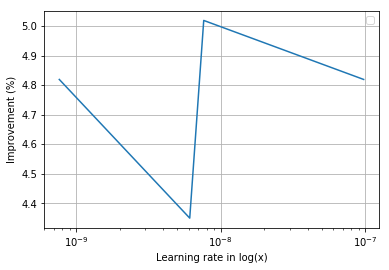
\includegraphics[width=.5\textwidth]{assets/appendix/plot_group25.png}
    \caption{Without batch normalization}
    \label{fig:ch_5_plot25}
\end{figure}
\begin{figure}[h]
    \centering
    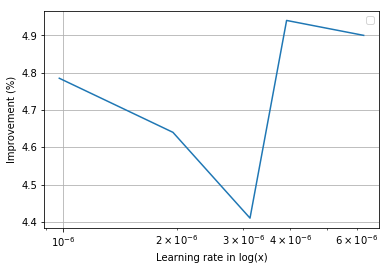
\includegraphics[width=.5\textwidth]{assets/appendix/plot_group21.png}
    \caption{With batch normalization}
    \label{fig:ch_5_plot21}
\end{figure}
\begin{figure}[h]
    \centering
    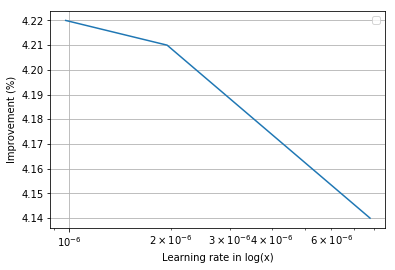
\includegraphics[width=.65\textwidth]{assets/appendix/plot_group23.png}
    \caption{Without batch normalization}
    \label{fig:ch_5_plot23}
\end{figure}
\begin{figure}[h]
    \centering
    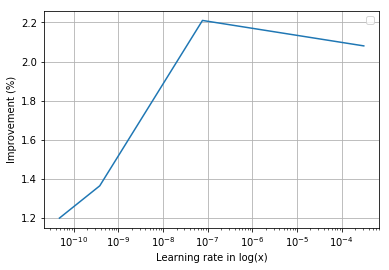
\includegraphics[width=.65\textwidth]{assets/appendix/plot_group1.png}
    \caption{Without batch normalization}
    \label{fig:ch_5_plot1}
\end{figure}
\begin{figure}[h]
    \centering
    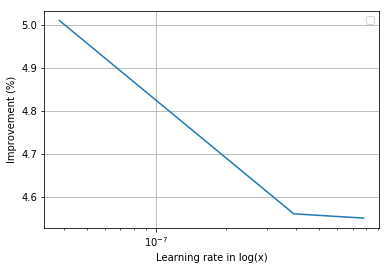
\includegraphics[width=.65\textwidth]{assets/appendix/plot_group5.png}
    \caption{Without batch normalization}
    \label{fig:ch_5_plot5}
\end{figure}

\chapter{Most significant variables according to feature selection}
\label{ch:appendix_c}
The following tables list the variables that best correlate with labeled output and may therefore possess potentially good discrimination capabilities. They were determined using the various feature selection algorithms introduced in Section \ref{sec:ch-4-input-vars}.

\npdecimalsign{.}
\nprounddigits{2}

\LTXtable{\textwidth}{assets/appendix/anova}
\LTXtable{\textwidth}{assets/appendix/rfe}
\LTXtable{\textwidth}{assets/appendix/fi}
